% unicodeは、hyperrefへの指定で、pdfのメタデータにあるタイトルの文字化けを防ぐ
% ptは細かい指定はできないらしい
% チートシート
% https://www.cpt.univ-mrs.fr/~masson/latex/Beamer-appearance-cheat-sheet.pdf
\documentclass[unicode, 14pt, aspectratio=169]{beamer} 
\usepackage{minted}
\usepackage{listings}
\usepackage{xcolor}
\usepackage{textcomp}
\usepackage[backend=biber, style=ieee]{biblatex}
\usetheme{rikako}
\date{\number\year 年\number\month 月\number\day 日}

\addbibresource{main.bib}
\title{runcのUNIXプログラミング}
\author{中村 遼太郎}
\begin{document}

\usemintedstyle{titech}
\begin{frame}[noframenumbering, plain]
\titlepage
\end{frame}
\section{導入}
\begin{frame}[t]
  \frametitle{runcってなに}
  後にDockerから独立した低レベルなコンテナランタイムのCLI
  % 左にレイヤの図。右に箇条書
  \begin{figure}
    \centering
    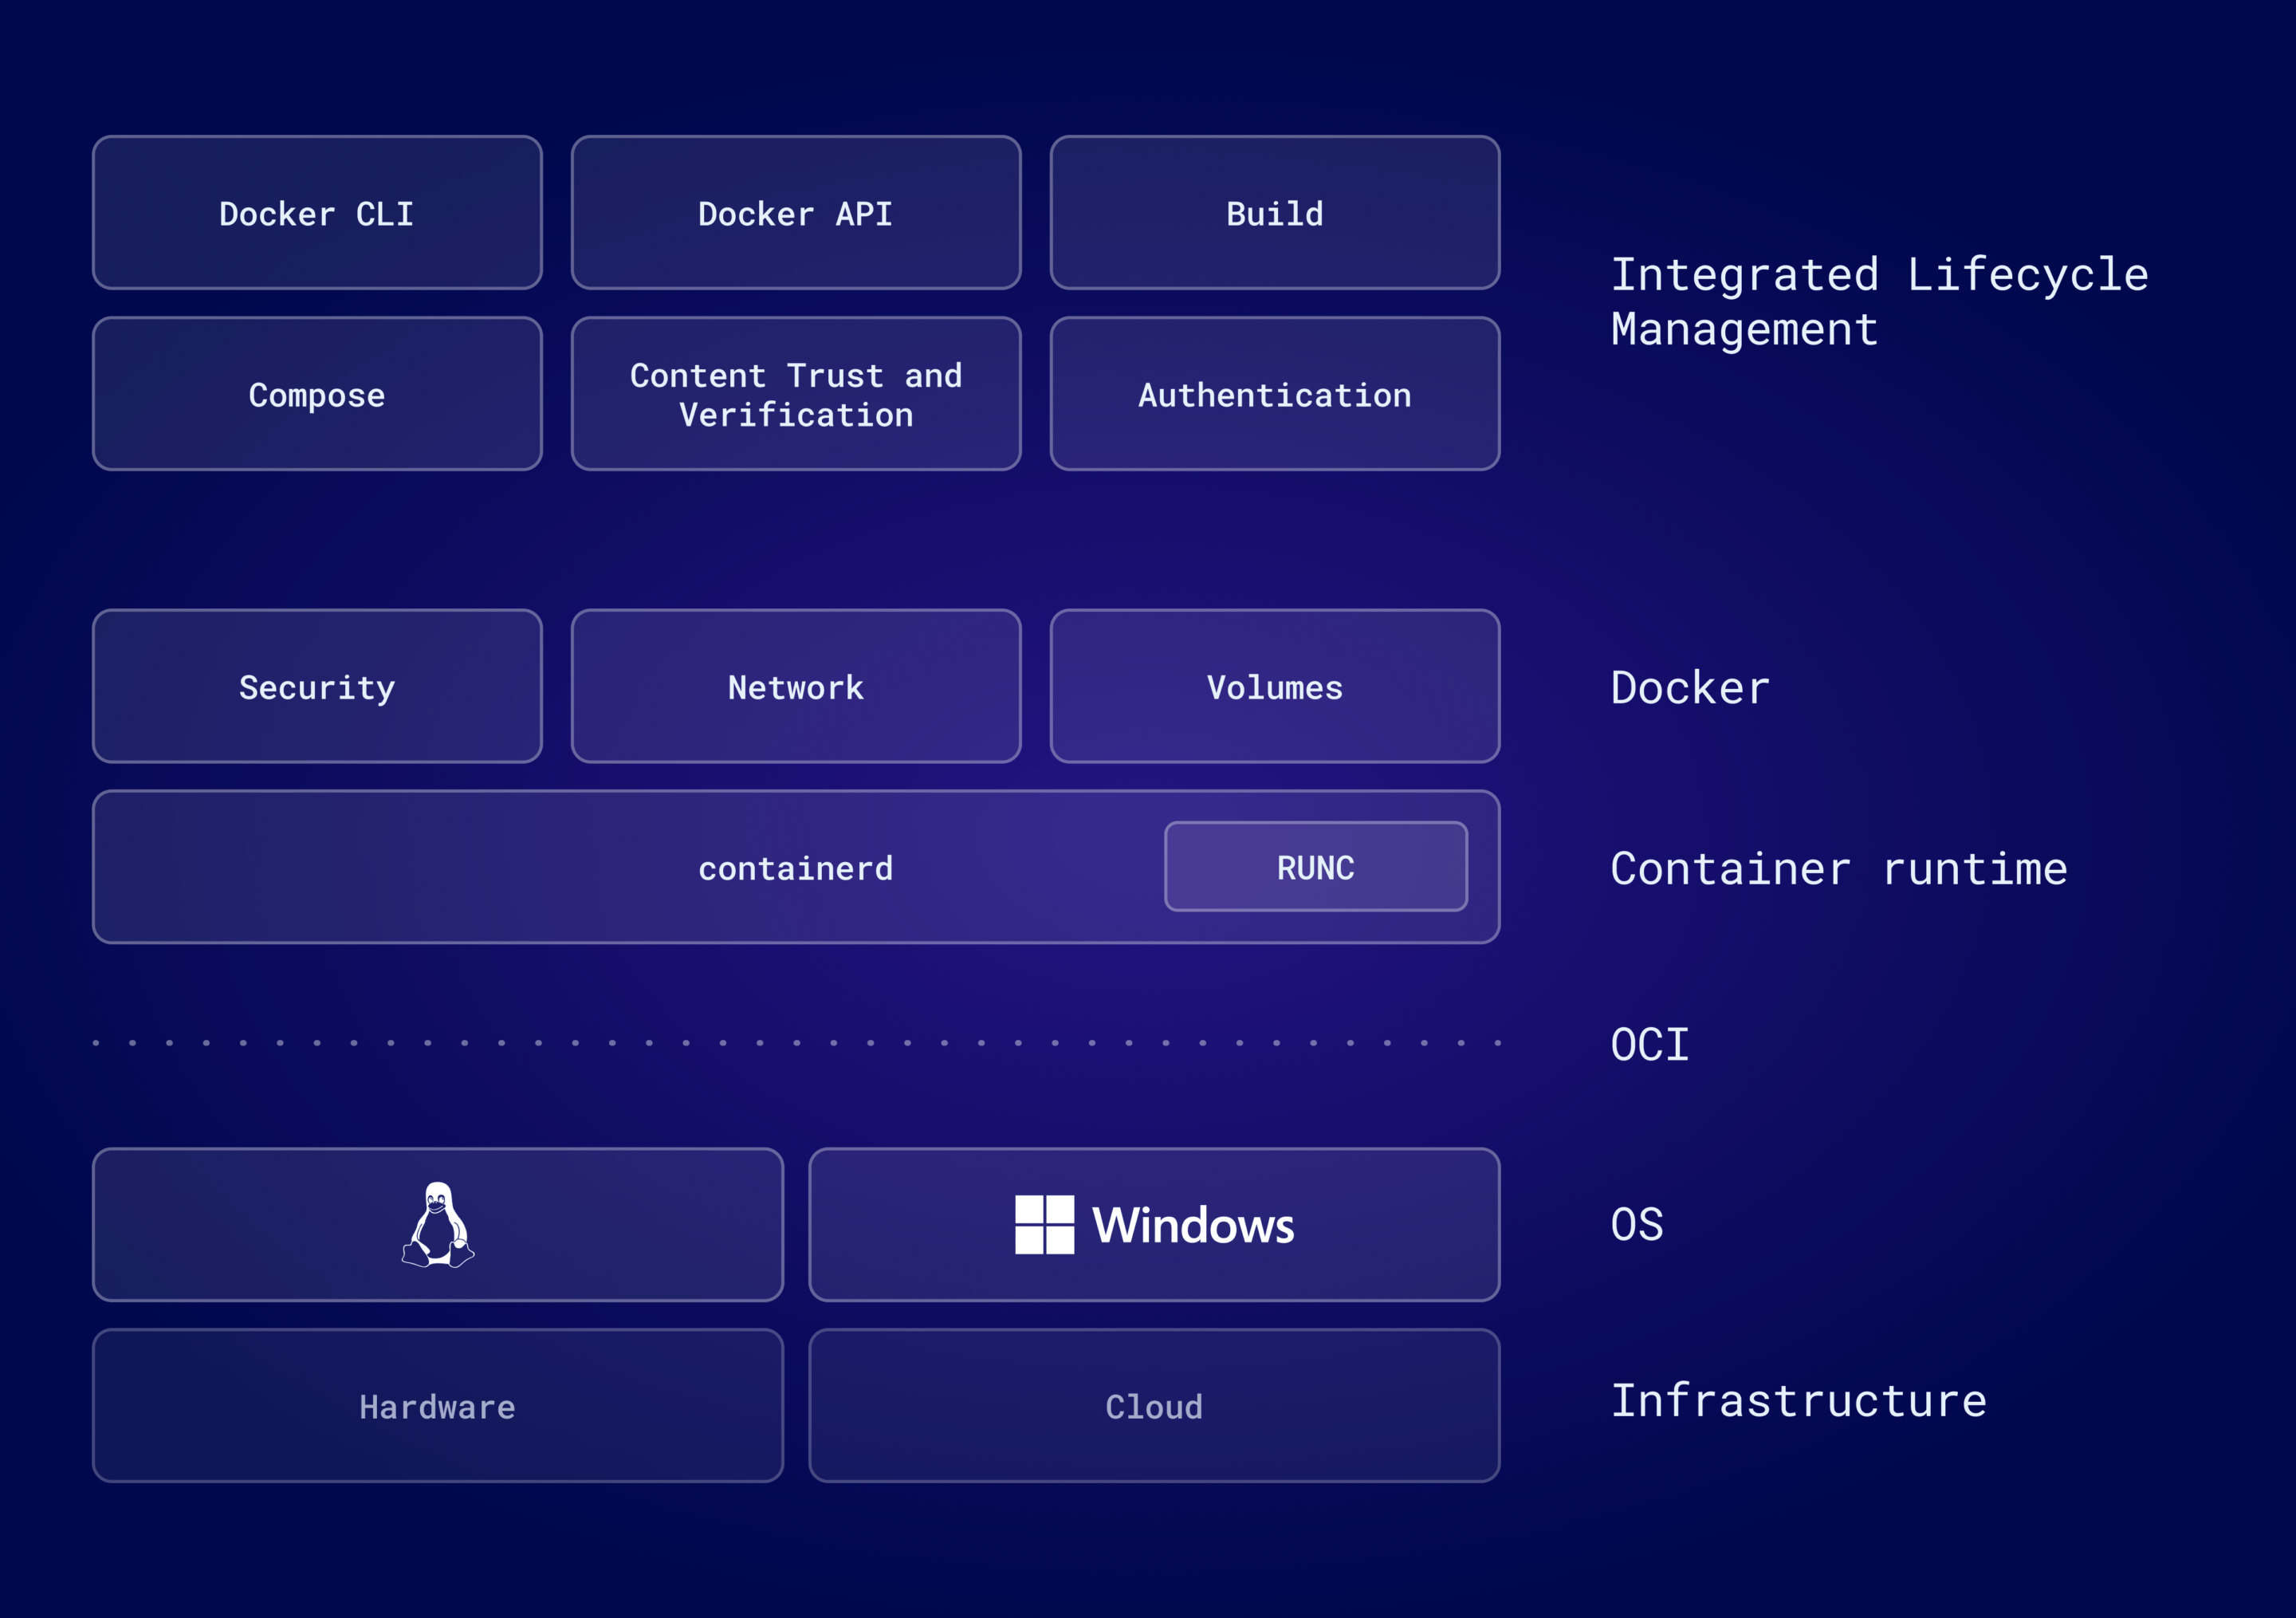
\includegraphics[width=6.5cm]{images/containerd-diagram-v1.png}
    \caption{Docker, runc, OSの階層\footnote{\scriptsize{\href{https://www.docker.com/blog/containerd-vs-docker}{containerd vs. Docker: Understanding Their Relationship and How They Work Together}より}}}
    \label{fig:runc}
  \end{figure}
\end{frame}
\begin{frame}[fragile=singleslide]
  \frametitle{イメージはいらない}
  コンテナのルート\texttt{/}があればいい
  \begin{center}
    \inputminted[fontsize=\footnotesize]{sh}{code/run.sh}
    runcでコンテナの\texttt{sh}を開始\supercite{runc}  
  \end{center}
\end{frame}
\begin{frame}[t]
  \frametitle{runcの設計}
  runcの実装はUNIXプログラミング
  \begin{center}
    Infrastructure Plumbing Manifesto\footnote{\scriptsize{Dockerのブログ \href{https://www.docker.com/blog/runc/}{Introducing runC: a lightweight universal container runtime
}より引用}}
    \end{center}
  \begin{quote}
    \begin{itemize}
    \item {\small When you need to create new plumbing, make it easy to re-use and contribute improvements back.}
    \item {\small Follow the unix principles: several simple components are better than a single, complicated one.}
    \item {\small Define standard interfaces which can be used to combine many simple components into a more sophisticated system.}
  \end{itemize}
  \end{quote}
\end{frame}
\begin{frame}[t]
  \frametitle{runc runの手続き}
  runが実行したrunc initがコンテナになる
  % 図を入れる
\end{frame}
\section{runc run}
\begin{frame}[t]
  \frametitle{コンテナ構造体のフィールド}
  設定、プロセス、状態、リソース制御
  % initプロセスか
  % stateDirにfifoをおく
  % _LIBCONTAINER_FIFOFD=でつたえる
  % fifoは、fifoではなくfd/以下のファイルを親プロセスでは読みにいってスタートしたか調べる。
  % fdの説明
\end{frame}
\begin{frame}[t]
  \frametitle{}
\end{frame}
\section{runc init}
\begin{frame}[t]
  \frametitle{a}
\end{frame}
% runcの寄贈
% https://www.docker.com/blog/runc/
% https://www.docker.com/blog/containerd-vs-docker/
% https://docs.docker.com/engine/daemon/alternative-runtimes/
\section{特徴}
\begin{frame}[t]
  \frametitle{特徴}
    単純なスライドにした。\textit{abc}
  \vspace{0.2\paperheight}
  \begin{itemize}
    \item 右下のnavigationを無効化\href{https://google.com}{doge}
    \item 各セクションの先頭に自動で目次を挿入
    \item frameが複数のスライドにまたいでも\\タイトルの末尾に番号をつけない
  \end{itemize}
\end{frame}

% \section{フォント}

\begin{frame}
\frametitle{採用したフォント}
\begin{itemize}
\item ヒラギノ
\item Helvetica Neue
\item Source Han Code JP
\item JetBrains Mono
\item STIX2
\end{itemize}
\end{frame}

\section{デモ}

\begin{frame}
  \frametitle{数式の例}
  \begin{equation}
    e^{i\theta} = \cos\theta + i\sin \theta \mathrm{sin}
  \end{equation}
\end{frame}

% \begin{frame}[fragile]
% \frametitle{コード}
%   {\small 
%     \begin{lstlisting}[language=C++]
% #include<bits/stdc++.h>
% using namespace std;

% int main() {
%   cout << "Hello World!" << endl;
%   return 0;
% }
%     \end{lstlisting}
% }
% \end{frame}

\begin{frame}[allowframebreaks]
  \frametitle{参考資料}
  \printbibliography
  % 引用していないbibファイルの要素も記載する  
  \nocite{*} 
\end{frame}

\end{document}
